\section{Appendix: Adding/Changing Maps}
\label{sec:appendix_maps}

As with all configuration, a local version is kept in the home folder of the user. The map files are loaded from the hidden folder '\textasciitilde/.compass/yourversion/data/maps' ('\textasciitilde' is the user's home directory, like /home/user).

\begin{figure}[H]
    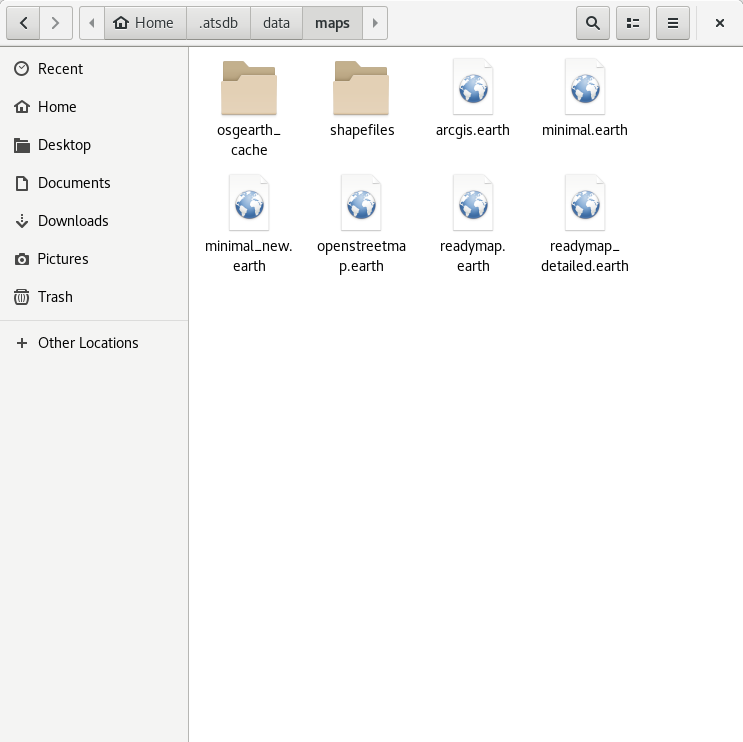
\includegraphics[width=10cm,frame]{figures/geoview_maps_config.png}
  \caption{Maps Folder}
\end{figure}

In this folder, the previosly discussed maps exist as osgEarth '.earth' files. If new .earth files are added, or the content of such files is changed, they can be used from the Geographic View after a restart.

\subsection{Map Example}
The easiest example is the 'minimal\_new.earth' file, which uses an ESRI shapefile from the subfolder 'shapefiles' to display the national borders.

\begin{lstlisting}
<map name="Wordwide Line Vectors" type="geocentric">
  
    <options>
        <lighting>false</lighting>
        <terrain>
            <min_tile_range_factor>8</min_tile_range_factor>
            <color>#000000FF</color>
        </terrain>
      
    </options>

    <feature_source name="world-data" driver="ogr">
        <url>shapefiles/TM_WORLD_BORDERS-0.3.shp</url>
        <convert type="line"/>
    </feature_source>
    
    <feature_model name="world_boundaries" feature_source="world-data">
        
        <layout tile_size="100000"  paged="true">
            <level max_range="1e10"/>
        </layout>
                
        <styles>
            <style type="text/css">
                world {
                   stroke:                   #ffff00;
                   stroke-width:             2px;
                   stroke-tessellation-size: 1km;
                   render-lighting:          false;
                   altitude-clamping:        none;
                   render-depth-test: false;
                }            
            </style>
        </styles>
        
    </feature_model>
 

</map>
\end{lstlisting}

\subsection{Editing Map Example}

The world background colour is set using the 'terrain color' tag. The name of the shapefile is given using the 'url' tag, the line colour and width is set in the style below. Basically a user can add their own files to the 'shapefiles' folder, and simply duplicate the 'feature\_model' part with their own ESRI shapefiles. This could the look like this:

\begin{lstlisting}
<map name="Wordwide Line Vectors" type="geocentric">
  
    <options>
        <lighting>false</lighting>
         <terrain color="#101010ff"/>
    </options>

    <feature_source name="world-data" driver="ogr">
        <url>shapefiles/TM_WORLD_BORDERS-0.3.shp</url>
        <convert type="line"/>
    </feature_source>
    
    <feature_model name="world_boundaries" feature_source="world-data">
        
        <layout tile_size="100000"  paged="true">
            <level max_range="1e10"/>
        </layout>
                
        <styles>
            <style type="text/css">
                world {
                   stroke:                   #ffff00;
                   stroke-width:             2px;
                   stroke-tessellation-size: 1km;
                   render-lighting:          false;
                   altitude-clamping:        none;
                   render-depth-test: false;                   
                }            
            </style>
        </styles>
        
    </feature_model>
  
    <feature_model name="doi">
        <features name="wolrd" driver="ogr">
            <url>shapefiles/doi.shp</url>
            <build_spatial_index>true</build_spatial_index>
            <ogr_driver>ESRI Shapefile</ogr_driver>
            <convert type="line"/>
        </features>        

        <layout tile_size="100000">
            <level max_range="1e10"/>
        </layout>

        <styles>
            <style type="text/css">
                states {
                   stroke:          #00ff00; 
                   stroke-width:    2px;
                   render-depth-test: false;
                }                    
            </style>
        </styles>        
    </feature_model>
</map>
\end{lstlisting}

\subsection{KML Feature Example}

While a number of formats are supported, to add a KML file, add the following part to a 'map' (as previously):

\begin{lstlisting}
     <feature_model name="wam_area">
        <features name="wam_area" driver="ogr">
            <url>shapefiles/wam_area.kml</url>
            <ogr_driver>LIBKML</ogr_driver>
            <build_spatial_index>true</build_spatial_index>
        </features>        

        <styles>
            <style type="text/css">
                states {
                   stroke:          #0000ff; 
                   stroke-width:    2px;
                   render-depth-test: false;
                }                    
            </style>
        </styles>        
    </feature_model>
\end{lstlisting}

\subsection{GML Feature Example}

To add a GML file, add the following part to a 'map' (as previously):

\begin{lstlisting}
   <model driver="feature_geom" name="gml" cache_enabled="false">
    <features driver="ogr">
	<ogr_driver>GML</ogr_driver>
        <url>shapefiles/example.gml</url>
        <caching_policy usage="no_cache"/>
    </features>
   </model>
\end{lstlisting}

\subsection{GeoTiff Feature Example}

To add a GeoTIFF file, add the following part to a 'map' (as previously):

\begin{lstlisting}
    <image driver="gdal" name="tiff" cache_enabled="false" visible="false">
        <url>/usr/share/osgearth/data/world.tif</url>
        <caching_policy usage="no_cache"/>
    </image>
\end{lstlisting}

\subsection{Graticule Example}

To add a graticule (latitude/longitude grid), add the following part to a 'map' (as previously):

\begin{lstlisting}
    <geodetic_graticule name="Graticule" visible="true">
        <color>#ffff007f</color>
        <label_color>#ffffffff</label_color>
        <grid_lines>20</grid_lines>
        <resolutions>10 5.0 2.0 1.0 0.5 0.25 0.125 0.0625 0.03125</resolutions>
    </geodetic_graticule>
\end{lstlisting}
\ \\

Please note that due to osgEarth constraints the graticule is not always displayed correctly. \\

\subsection{Offline OpenStreetMap Example}

There exist a number of options how OpenStreetMap maps can be made available in an offline environment. The most convinient option the author found was using the QGIS tool (\href{https://www.qgis.org/}{Link}), which should be available in all common Linux distributions. \\

Using this tool, OpenStreetMap tiles can be downloaded and saved in a number of formats. To allow for efficient usage, the MBTiles format was used successfully. In this format, OpenStreetMap (and other online tile-based maps) can be stored in a single file and transferred to an offline environment.

\subsubsection{Use QGIS to Generate MBTiles Map}

In this example description, QGIS 3.22 was used. First, QGIS is start in an environment with internet access. Then, OpenStreetMap is selected as background layer by double-clicking on XYZ Tiles $\rightarrow$ OpenStreetMap).

\begin{figure}[H]
    \hspace*{-2cm}
    \includegraphics[width=18cm,frame]{figures/qgis_osm1.png}
\end{figure}

Then, XYZ tiles are written as MBTiles using the 'Processing' toolbox, which is started/displayed using the menu bar 'Processing' $\rightarrow$ 'Processing' (or already displayed in the bottom right. \\

If the menu entry is missing, it has to be activated once using the menu bar 'Plugins' $\rightarrow$ 'Manage and Install Plugins' dialog (find 'Processing' entry and check the checkbox). \\

After this step, input 'xyz tiles' in the Processing toolbox search window.

\begin{figure}[H]
    \hspace*{-2cm}
    \includegraphics[width=18cm,frame]{figures/qgis_osm2.png}
\end{figure}

Double-click the entry 'Generate XYZ Tiles (MBTiles)' to start the following dialog.

\begin{figure}[H]
    \includegraphics[width=12cm,frame]{figures/qgis_osm3.png}
\end{figure}

The following (important) options can be set:
\begin{itemize}
 \item Extend: Latitude/Longitude bounding rectangle to export
 \item Minimum zoom: Minimum level of detail, e.g. 1
 \item Maxmimum zoom: Maximum level of detail, e.g. 12-15 (changes creation time and resulting file size)
 \item Tile Format: Graphics for using, e.g. JPG (to reduce file size)
 \item Output file: MBTiles file to be written
\end{itemize}
 \ \\

Please note that for higher level of details, the application crashed with a SQLite locked error message. This can be mitigated (might not be required in newer versions of QGIS) using the menu bar 'Settins' $\rightarrow$ 'Options' dialog. In the top left search bar 'threads' can be entered to then change the 'Max Threads' variable to '1'. \\

\begin{figure}[H]
    \includegraphics[width=14cm,frame]{figures/qgis_osm4.png}
\end{figure}
 
After these options were set, the 'Run' button can be clicked. \\

Please review and consider the OpenStreetMap copyright and license when creating such offline maps (\href{https://www.openstreetmap.org/copyright}{Link}). \\

After successful complete of this task, the resulting MBTiles file has to be copied to any \textasciitilde'/.compass location and be used in a .earth file like the following:

\begin{lstlisting}
<map name="OpenStreetMap" type="projected" version="2">

    <options>
        <lighting>false</lighting>
        <profile>spherical-mercator</profile>
        <terrain tile_size="2" morph_imagery="false" range_mode="PIXEL_SIZE_ON_SCREEN" tile_pixel_size="512" color="#000000FF"/>
    </options>
    
    <MBTilesImage name="OSM">
        <filename>../../../osm/qgis12.mbtiles</filename>
    </MBTilesImage>
    
</map>
\end{lstlisting}

Then such a map is selected in the Geographic View, only in the selected QGIS extend map data is available.

\begin{figure}[H]
    \hspace*{-2.5cm}
    \includegraphics[width=19cm,frame]{figures/geoview_qgis_osm1.png}
\end{figure}

Such a map could be enhanced by combining it with the minimal\_2d.earth map, to overlay national border - to give location awareness where no OpenStreetMap data is available.

\begin{lstlisting}
<map name="OpenStreetMap" type="projected" version="2">

    <options>
        <lighting>false</lighting>
        <profile>spherical-mercator</profile>
        <terrain tile_size="2" morph_imagery="false" range_mode="PIXEL_SIZE_ON_SCREEN" tile_pixel_size="512" color="#000000FF"/>
    </options>
    
    <feature_model name="world boundaries">
        <features name="world boundaries" driver="ogr">
            <url>shapefiles/TM_WORLD_BORDERS-0.3.shp</url>
        </features>       
        
        <styles>
            <style type="text/css">
                states {
                   stroke:                   #ffff00;
                   stroke-width:             2px;
                   render-lighting:          false;
                   stroke-tessellation-size: 1km;
                   altitude-clamping:   terrain-gpu;
                   render-depth-offset:      true;     
                }                    
            </style>
        </styles>        
    </feature_model>
    
    <feature_model name="Airports Europe">
        <features name="Airports Europe" driver="ogr">
            <url>shapefiles/AIRP_PT_2013.shp</url>
            <build_spatial_index>true</build_spatial_index>
        </features>       
        
        <layout>
            <level name="far"    style="large"  max_range="1e10"/>
            <level name="medium" style="medium" max_range="3000000"/>
            <level name="close"  style="small"  max_range="500000"/>
        </layout>

        <styles>
            <selector name="large" class="label-large">
                <query>
                    <expr> <![CDATA[ AIRP_PASS = 2 ]]> </expr>
                </query>
            </selector>
            
            <selector name="medium" class="label-medium">
                <query>
                    <expr> <![CDATA[ AIRP_PASS = 1 ]]> </expr>
                </query>
            </selector>
            
            <selector name="small" class="label-small">
                <query>
                    <expr> <![CDATA[ AIRP_PASS = 0 ]]> </expr>
                </query>
            </selector>
            
            <style type="text/css">   
                label {
                    text-declutter: true;
                    text-content:   [AIRP_ICAO_];
                    text-encoding:  utf-8;
                    text-align:     right_right;
                    text-priority:  [AIRP_PASS];
                    text-halo:      #2f2f2f;
                }                
                label-large : label {
                    text-size:      18.0;
                    text-color: #ffffff;
                    icon: "../icons/placemark.png";
                    icon-scale:      0.7;
                }
                label-medium : label {
                    text-size:      16.0;
                    text-color: #eeeeee;
                    icon: "../icons/placemark.png";
                    icon-scale : 0.6;
                }           
                label-small : label {
                    text-size:      14.0;
                    text-color: #dddddd;
                    icon: "../icons/placemark.png";
                    icon-scale : 0.5;
                }
            </style>
        </styles>
    </feature_model>
    
    
    <MBTilesImage name="OSM">
        <filename>../../../osm/qgis12.mbtiles</filename>
    </MBTilesImage>

    
</map>

\end{lstlisting}

\begin{figure}[H]
    \hspace*{-2.5cm}
    \includegraphics[width=19cm,frame]{figures/geoview_qgis_osm2.png}
\end{figure}

 
\subsection{Others}

For further information please refer to the osgEarth user manual \url{https://buildmedia.readthedocs.org/media/pdf/osgearth/latest/osgearth.pdf}, e.g. in Section Features \& Symbology.
 
